\subsection{Infinite plate with a circular hole}
\paragraph{}
In this example, an infinite plate with a traction free hole under uniaxial tension $(\sigma = 1 N/m^2 )$
along x-axis (see fig.~\ref{qdt_fig:ex_chole_geo_bc}) is considered.

    \begin{figure}[h!]
        \centering
        \scalebox{0.75}{
            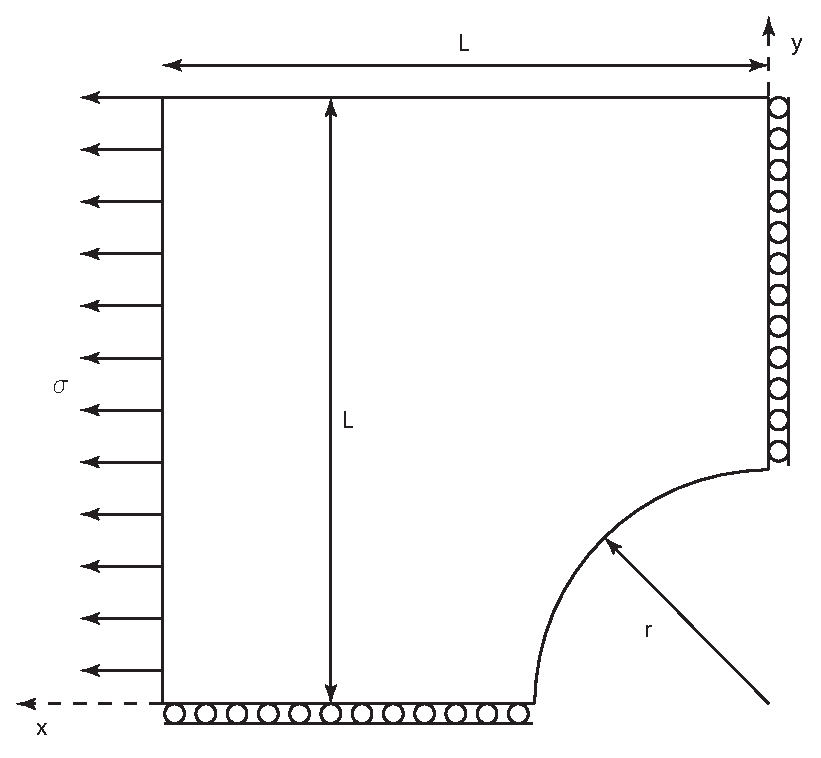
\includegraphics{quadtree/ex_images/qdt_chole_quat_geo_bc.eps}
        }
        \caption{ Infinite plate with a circular hole: geometry and boundary conditions}
        \label{qdt_fig:ex_chole_geo_bc}
    \end{figure}
    
The exact solution of the principal stresses in Cartesian coordinate $(r,\theta)$ is given by \cite{Sukumar2001} in eq.~\ref{iso_eq:ex_chole_stress_sol}.
where $a$ is the radius of the hole.
The material properties are: Young’s modulus $E = 100 N/m^2$ and Poisson’s ratio $\nu = 0.3$.
The closed form displacement in Cartesian coordinate is given in eq.~\ref{iso_eq:ex_chole_disp_sol}.

\paragraph{}

Generated background mesh, coloring and the final result with $res=32$, $s_{max}=16$ and $s_{min}=1$ are shown in fig.~\ref{qdt_fig:ex_cantilever_beam_background_mesh}, fig.~\ref{qdt_fig:ex_cantilever_beam_mesh_coloring} and fig.~\ref{qdt_fig:ex_cantilever_beam_mesh_final}.

%%
The geometry is: length $L=8m$, height $D=4m$.
The material properties are: Young’s modulus $E$ = $3 \times 10^7 N/m^2$ , Poisson’s ratio $ \nu =0.25$.
The parabolic shear force is $P = 250 N$.
The exact solutions for the displacements are given by \cite{Aug2008} as eq.~\ref{iso_eq:cantilever_beam_displacement_solution}.
where $I=D^3/12$ is the moment of inertia, $\mean{E}=E$, $\mean{\nu}=\nu$ and $\mean{E}=E/(1-\nu^2)$, $\mean{\nu}=nu/(1-nu)$ for plane stress and plane strain condition respectively.
The stress $\sigma$ can be expressed as \cite{Aug2008} as eq.~\ref{iso_eq:cantilever_beam_stress_solution}.
The strain energy can be derived from eq.~\ref{iso_eq:cantilever_beam_stress_solution} and eq.~\ref{iso_eq:cantilever_beam_displacement_solution} as eq.~\ref{iso_eq:cantilever_beam_energy_solution}.

\paragraph{}
In this example, rigid body motion is constrained by fixing 3 DOF on the left edge of the beam.
$u_x=0$ for points at $(0,-D/2)$ and $(0,D/2)$ and $u_y =0$ for point at $(0,0)$.
Stress from analytical solution in eq.~\ref{iso_eq:cantilever_beam_stress_solution} are applied on the boundary.

\paragraph{}
Due to the fact that the geometry of the cantilever beam can be described by four points and four straight lines, drawing in AutoCAD may not be necessary.
As a result, the input geometry is defined manually.
Generated background mesh, coloring and the final result with $res=32$, $s_{max}=16$ and $s_{min}=1$ are shown in fig.~\ref{qdt_fig:ex_cantilever_beam_background_mesh}, fig.~\ref{qdt_fig:ex_cantilever_beam_mesh_coloring} and fig.~\ref{qdt_fig:ex_cantilever_beam_mesh_final}.
%%

\begin{figure}
    \centering
    \scalebox{0.6}{
        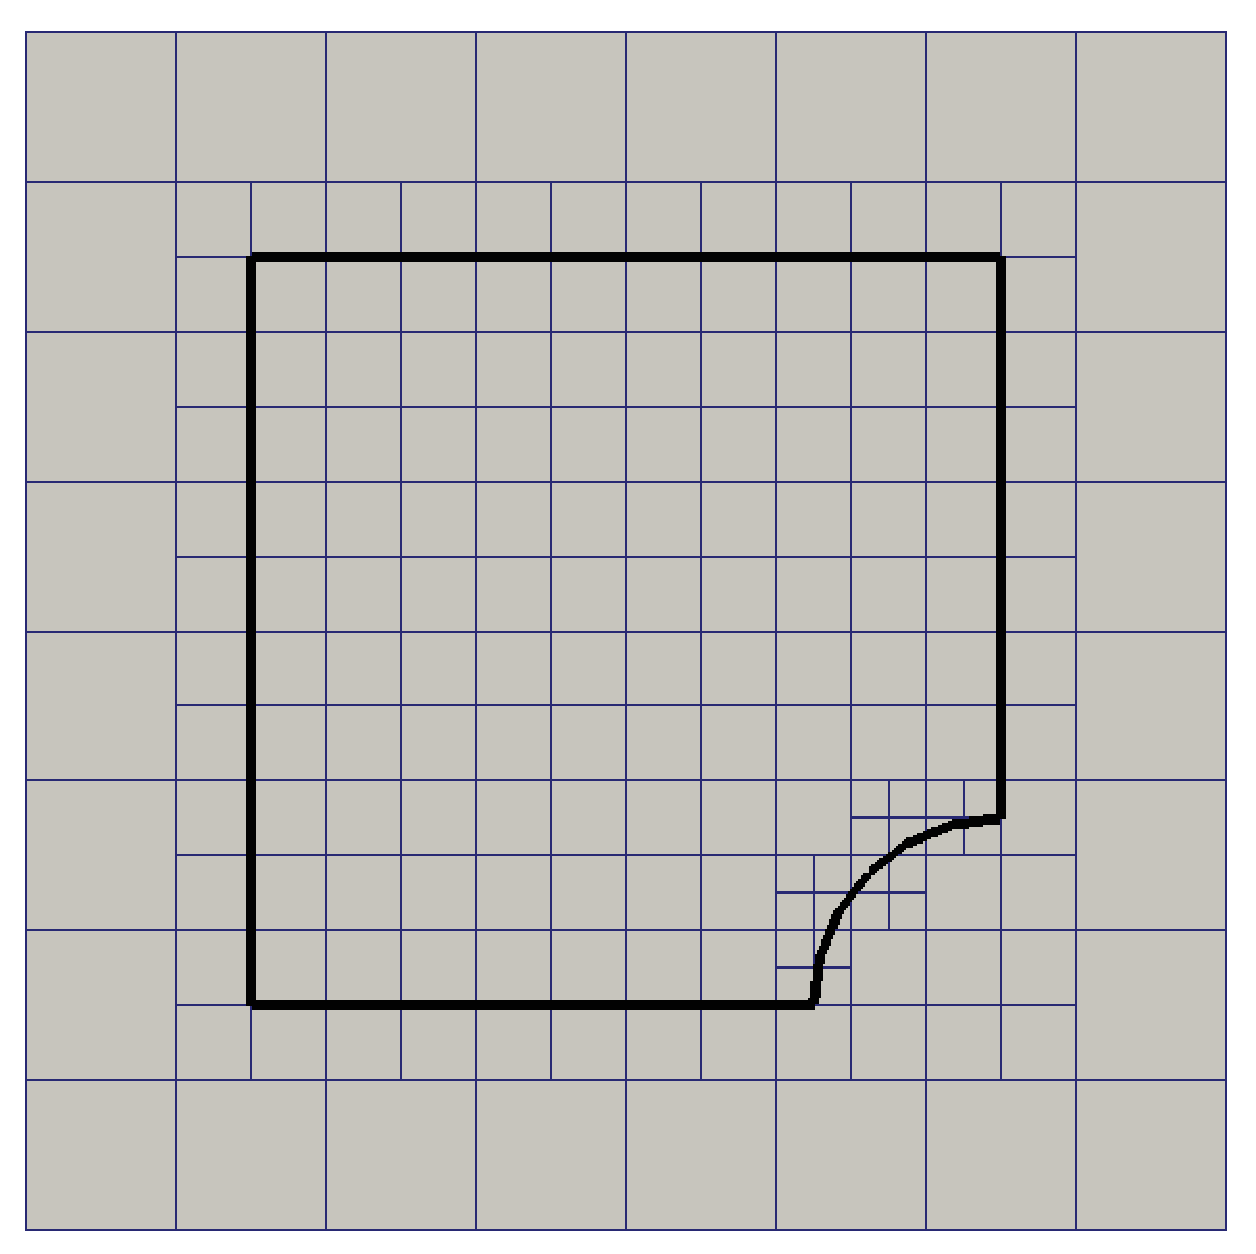
\includegraphics{quadtree/ex_images/ex_chole_background.eps}
    }
    \caption[Background mesh of infinite plate with a circular hole]{Background mesh of infinite plate with a circular hole : Bold lines represents the input geometry}
    \label{qdt_fig:ex_chole_background_mesh}
\end{figure}

\begin{figure}
    \centering
    \scalebox{0.6}{
        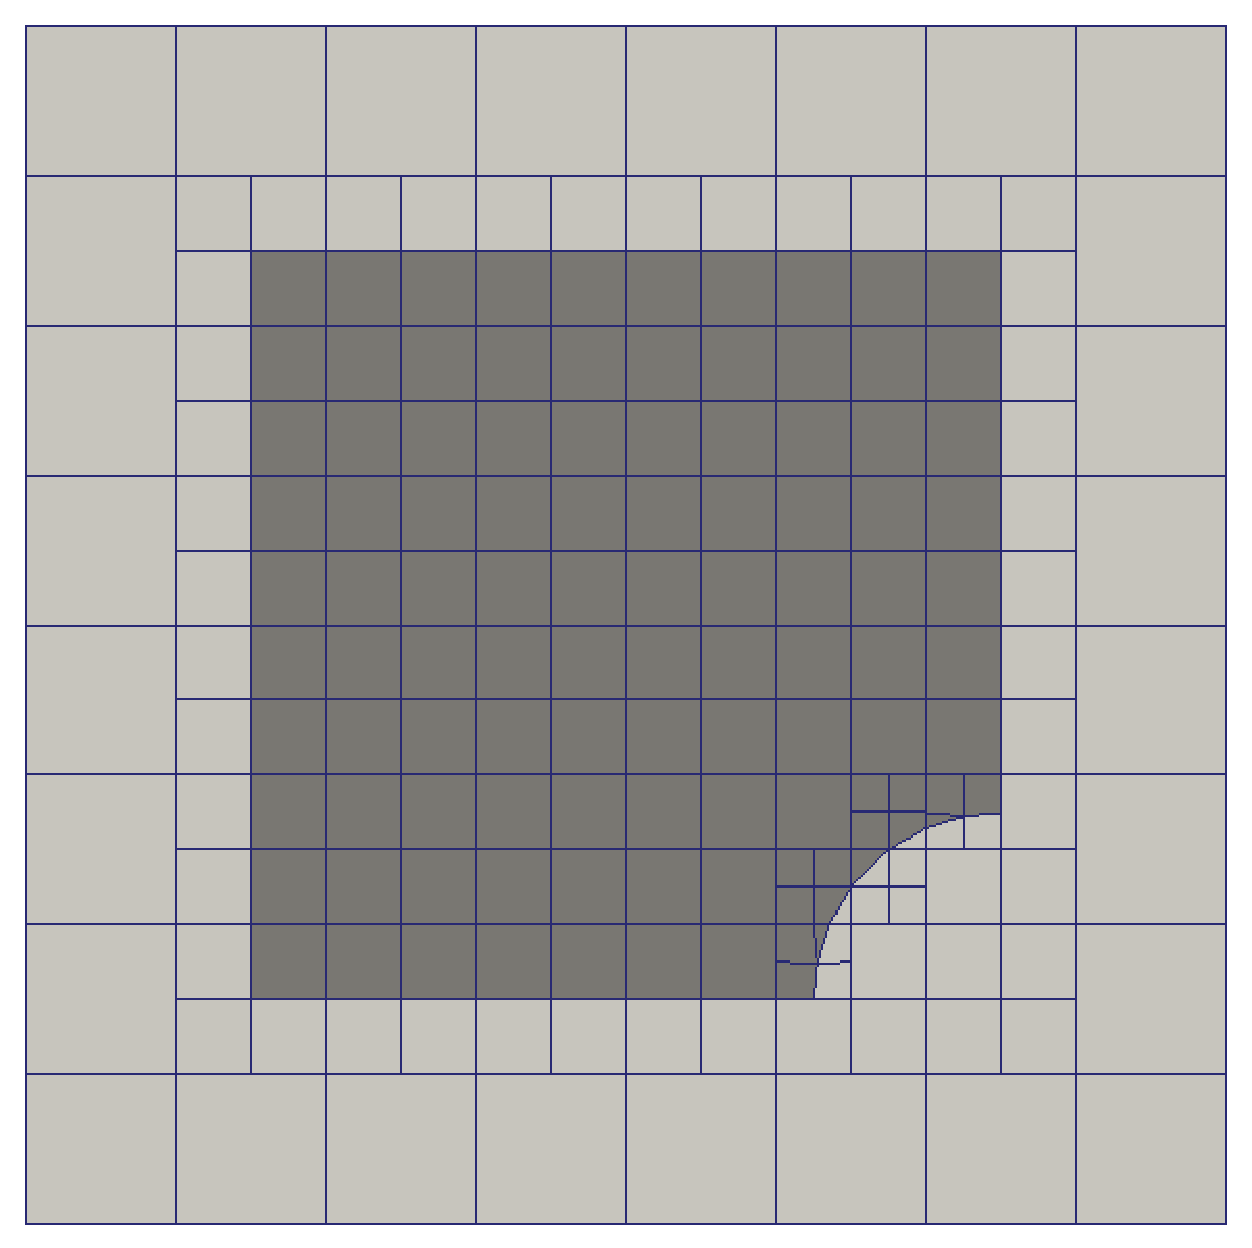
\includegraphics{quadtree/ex_images/ex_chole_coloring.eps}
    }
    \caption[Mesh coloring of infinite plate with a circular hole]{Mesh coloring of infinite plate with a circular hole : Grey area represents the cantilever beam}
    \label{qdt_fig:ex_chole_mesh_coloring}
\end{figure}

\begin{figure}
    \centering
    \scalebox{0.5}{
        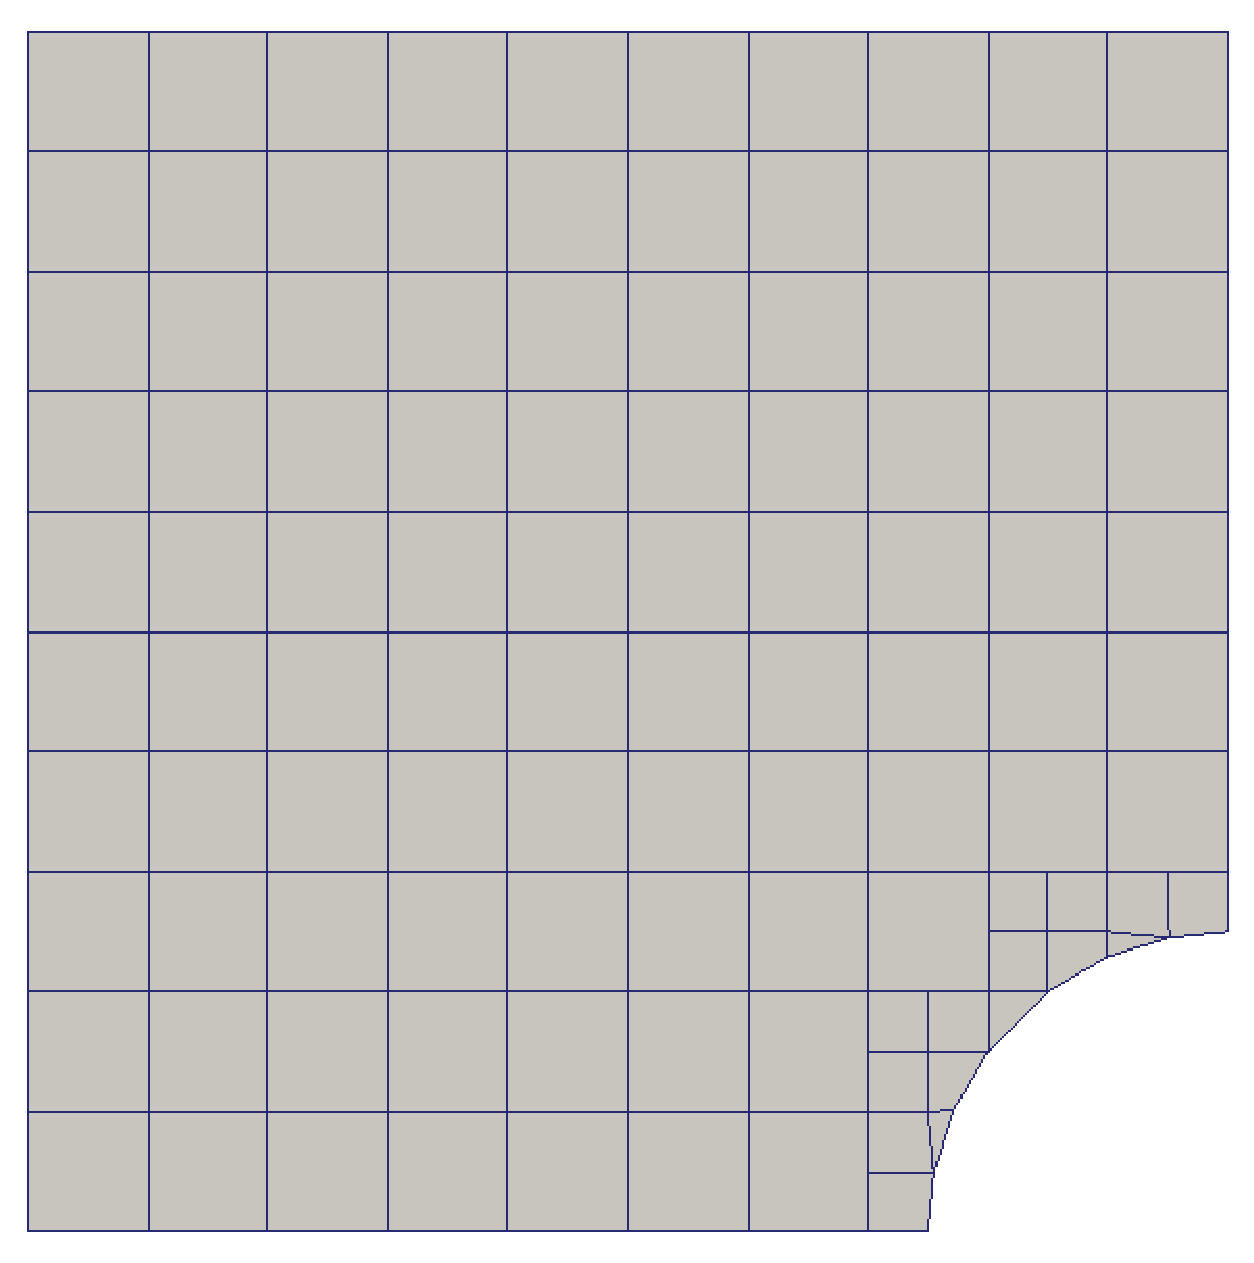
\includegraphics{quadtree/ex_images/ex_chole_mesh_262.eps}
    }
    \caption[Final mesh of infinite plate with a circular hole]{Final mesh of infinite plate with a circular hole}
    \label{qdt_fig:ex_chole_mesh_final}
\end{figure}
% 262 - 0.0112 (32-4/5-4)
% 290 - 0.0101 (64-4/5-4)
% 876 - 0.0036216 (128-4/8-4)
% 3280- 0.0010068 (256-4/15-4)
\begin{figure}[!ht]
    \begin{subfigure}[b]{1\linewidth}
        \centering
        \scalebox{0.4}{
            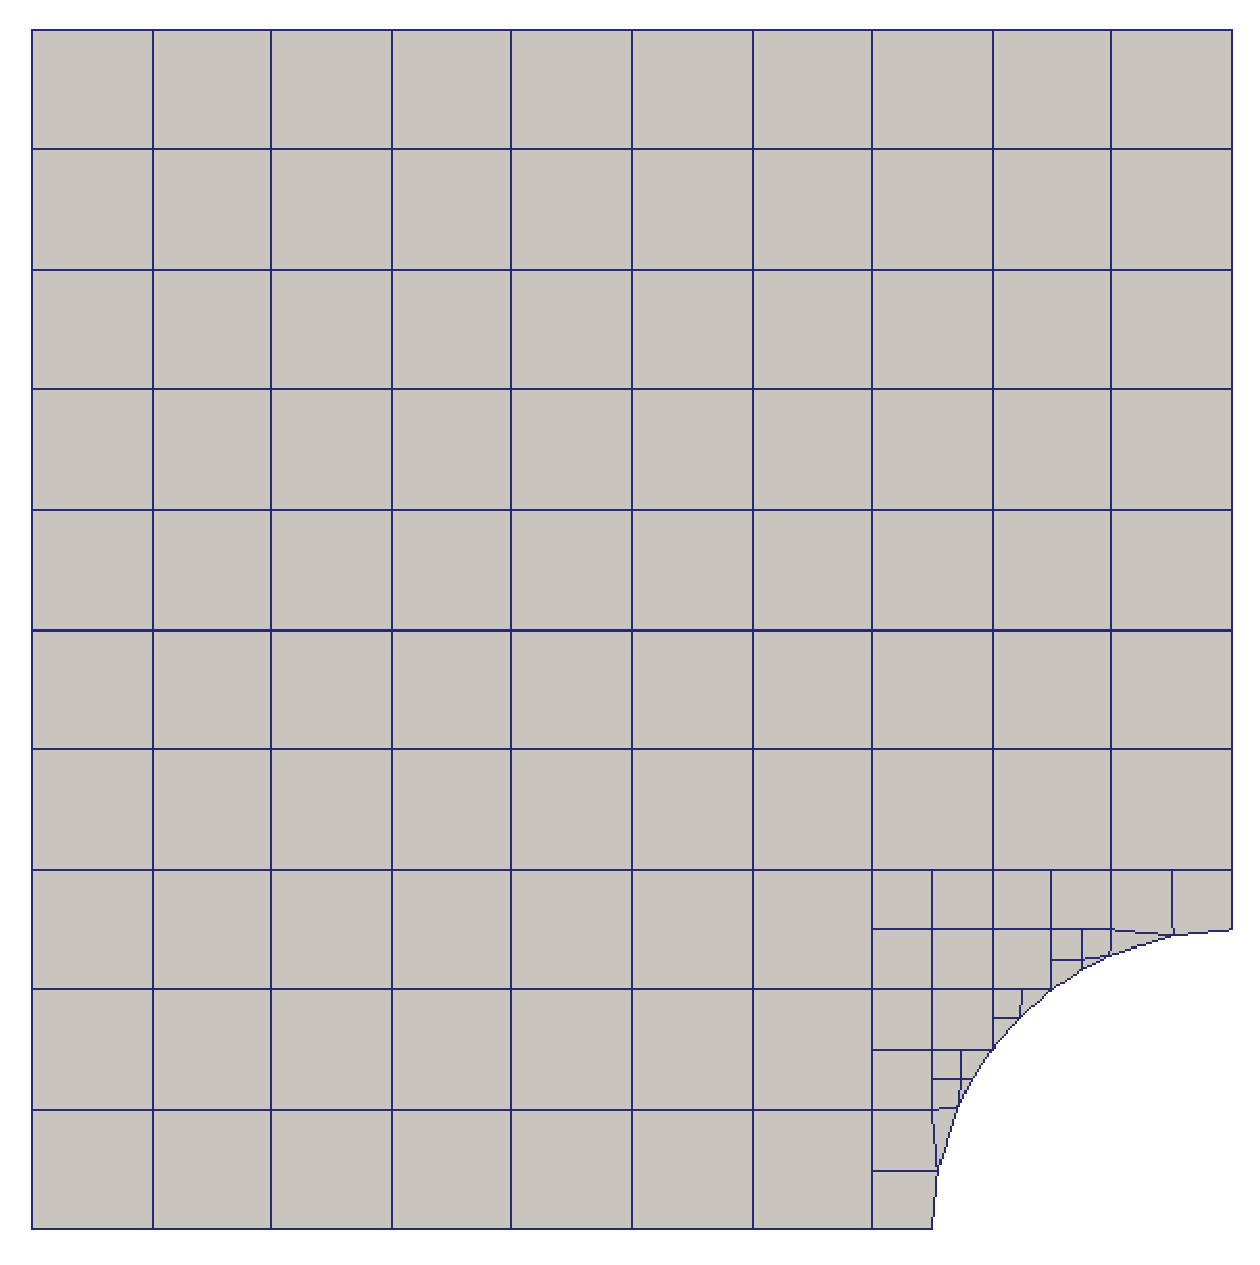
\includegraphics{quadtree/ex_images/ex_chole_mesh_290.eps}
        }
        \caption{Mesh with $res=64$, $s_{max}=4$, 290 DOFs}
    \end{subfigure}
    \\
    \begin{subfigure}[b]{1\linewidth}
        \centering
        \scalebox{0.4}{
            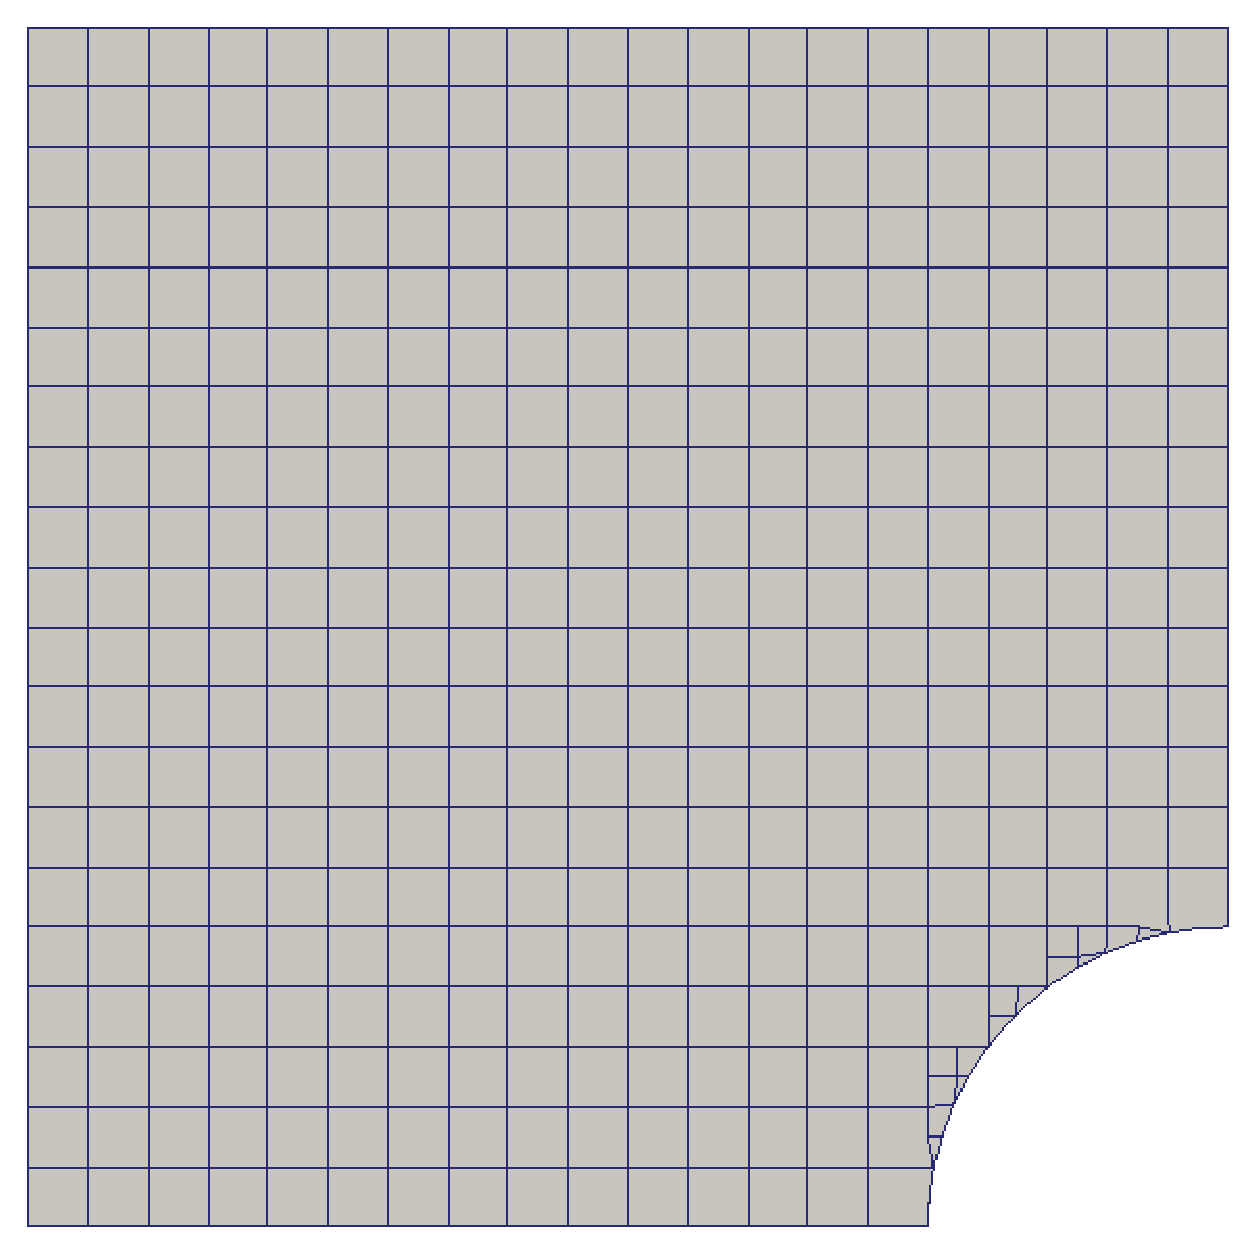
\includegraphics{quadtree/ex_images/ex_chole_mesh_876.eps}
        }
        \caption{Mesh with $res=128$, $s_{max}=4$, 876 DOFs}
    \end{subfigure}
\end{figure}

\begin{figure}[!ht]\ContinuedFloat
    \begin{subfigure}[b]{1\linewidth}
        \centering
        \scalebox{0.5}{
            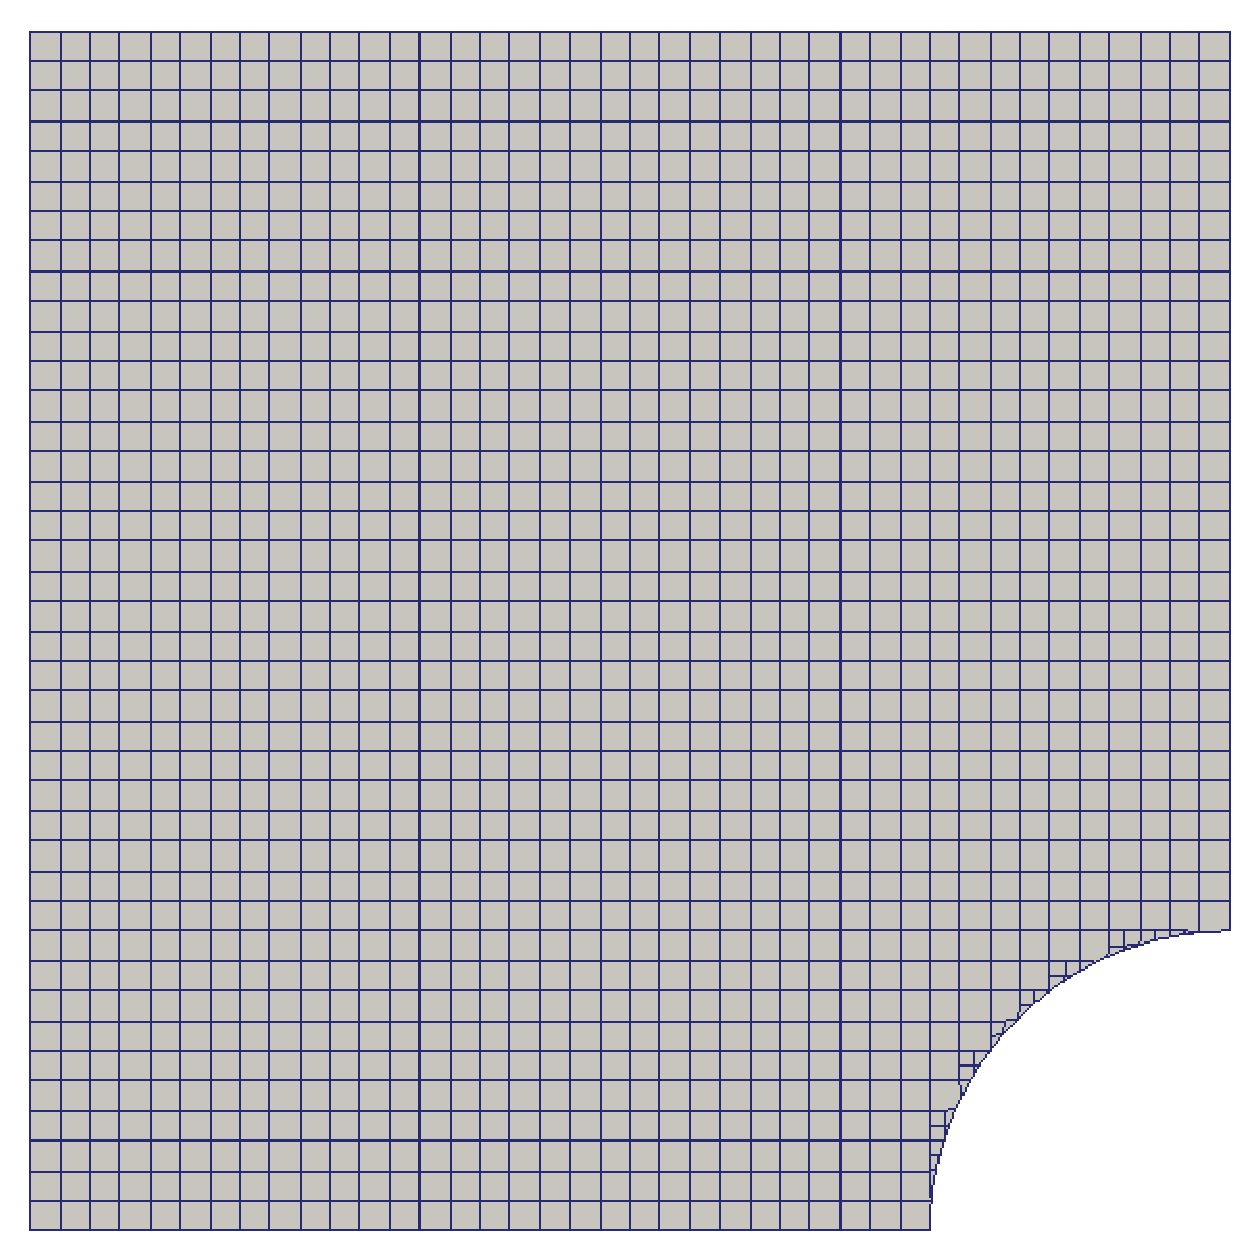
\includegraphics{quadtree/ex_images/ex_chole_mesh_3280.eps}
        }
        \caption{Mesh with $res=256$, $s_{max}=4$, 3280 DOFs}
    \end{subfigure}
    \caption[Mesh of the infinite plate with a circular hole]{Mesh of infinite plate with a circular hole}
    \label{qdt_fig:ex_chole_mesh_all}
\end{figure}


\begin{figure}[!ht]
    \centering
    \scalebox{0.75}{
        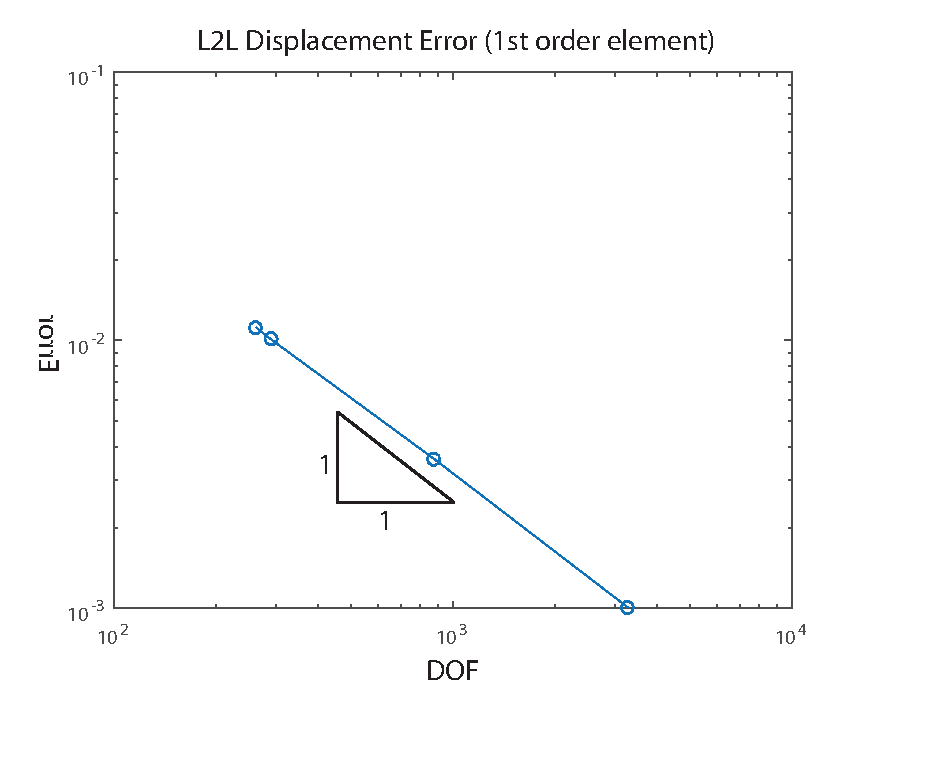
\includegraphics{quadtree/ex_images/ex_chole_conv.eps}
    }   
    \caption[Convergence of the infinite plate with a circular hole]{Convergence of the infinite plate with a circular hole}
    \label{qdt_fig:ex_chole_mesh_conv}
\end{figure}